\documentclass[border=10pt]{standalone}
\usepackage{tkz-fct}
\usepackage{tkz-base}
\usepackage{array}

\begin{document}

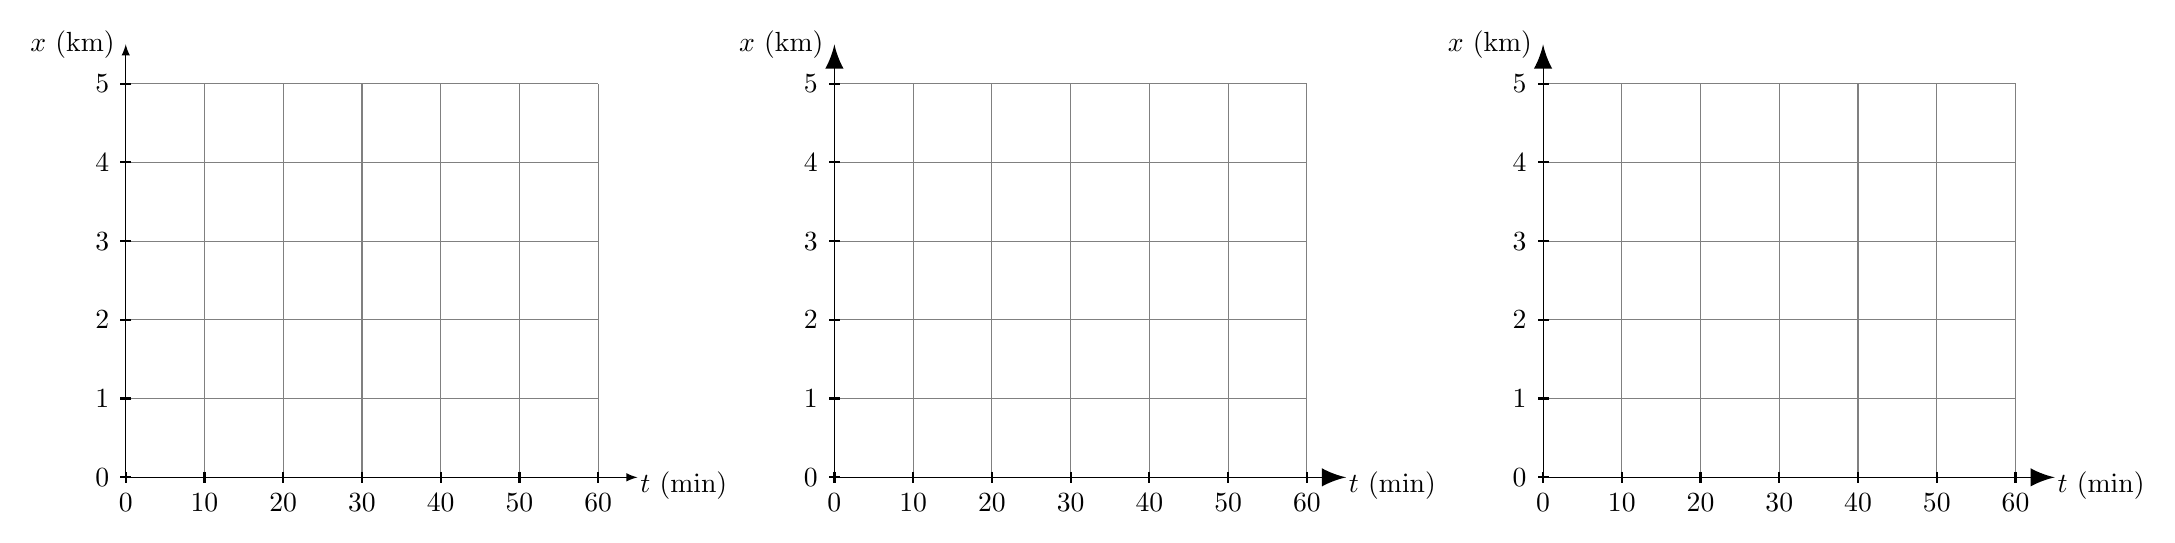
\begin{tikzpicture}
% Tableau en LaTeX standard avec tkz-text

% Repère quadrillé
\tkzInit[xmin=0,xmax=60,xstep=10,ymin=0,ymax=5, ystep=1]
\tkzGrid
\tkzDrawX[label = $t$ (min), right]
\tkzDrawY[label = $x$ (km)]
\tkzLabelXY
\tkzFct[line width=2pt, domain=0:60]{(-5/60.)*\x +5}
\begin{scope}[xshift=9cm]
  \tkzInit[xmin=0,xmax=60,xstep=10,ymin=0,ymax=5, ystep=1]

\tkzGrid
\tkzLabelXY

\tkzDrawX[label = $t$ (min), right]
\tkzDrawY[label = $x$ (km)]
\tkzFct[line width=2pt, domain=0:60]{(5/30.)*\x}
\end{scope}
\begin{scope}[xshift=18cm]
  \tkzInit[xmin=0,xmax=60,xstep=10,ymin=0,ymax=5, ystep=1]

\tkzGrid
\tkzLabelXY

\tkzDrawX[label = $t$ (min), right]
\tkzDrawY[label = $x$ (km)]
\tkzFct[line width=2pt, domain=0:60]{5}
\end{scope}
\end{tikzpicture}

\end{document}
